\documentclass[dvipdfmx, tikz]{standalone}

\usetikzlibrary{backgrounds}
\usetikzlibrary{arrows.meta}
\usetikzlibrary{shapes.multipart}

\begin{document}
  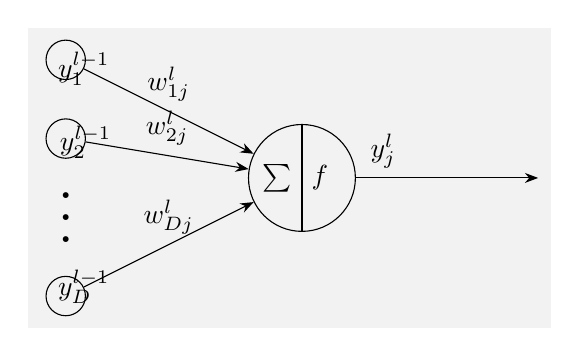
\begin{tikzpicture}[
    background rectangle/.style={fill=white!95!black},
    show background rectangle,
    neuron/.style={draw, circle, minimum width=0.5cm},
    >=Stealth, every node/.style={shape border uses incircle}]

    \def\ysep{1cm}

    \node [draw, circle split, minimum width=1cm, rotate=90] (q) at (3, -1.5 * \ysep)
      {\rotatebox{-90}{$\sum$} \nodepart{lower} \rotatebox{-90}{$f$}};

    \draw [->] (q) -- node [pos=0.15, above] {$y_{j}^{l}$} ++(3cm, 0);

    \foreach \i/\j in {1/1, 2/2, 4/D} {
      \node [neuron] (p1\i) at (0, {(-\i + 1) * \ysep}) {};
      \draw [->] (p1\i)
        -- node [pos=0] {$y_{\j}^{l-1}$}
           node [pos=0.5, above] {$w_{\j j}^{l}$} (q);
    }
    \node [scale=2, yshift=3] at (0, -2 * \ysep) {$\vdots$};
  \end{tikzpicture}
\end{document}
